\section{Related Work}

\subsection{Creative Live Streaming}
Perhaps the three most popular genres for live streams are video gaming \cite{Pellicone2017, Lessel2017, Sjoblom2017, Hamilton2014}, programming \cite{Faas2018, Haaranen2017}, and lifestyle \cite{Lu2018a, Tang2016}. Popular live streaming platforms that host a variety of live stream genres include Twitch, YouTube, Facebook, Instagram, and Periscope. Creative live streams can be found on all of these platforms, but platforms dedicated specifically to \textit{creative} live streaming have also emerged, such as Picarto, Pixiv Sketch, and Behance \footnote{\href{www.picarto.tv}{\nolinkurl{picarto.tv}}, \href{https://sketch.pixiv.net/lives}{\nolinkurl{sketch.pixiv.net/lives}}, \href{https://behance.net/live}{\nolinkurl{behance.net/live}}}.

Live streaming democratizes the studio-apprentice model, enabling anyone to see experts' in-context choices by working alongside them \cite{Schon1985}. Section \ref{sec:liveclips_formative} of this chapter describes the motivations and challenges of both streamers and viewers of creative live streams, comparing and contrasting them with prior work on live streaming in other domains. We use Twitch's definition of creative work: ``visual art, woodworking, costume creation, prop building, music composition, or any other process in which you entertain and connect around a creative activity'' \cite{Moorier2015}. These activities focus on creating a novel artifact, unlike typical video games or lifestyle streaming.

\subsection{Examples are Important for Creative Inspiration}
Searching and browsing examples is an important part of the creative process \cite{Shneiderman2002, Shneiderman2007, Greene2002, Herring2009, Muller-Wienbergen2011, Bawden1986}. 
While search engines are a common tool for finding examples, directed search can prevent serendipitous discovery \cite{Benjamin2014}. Happening upon an unexpected or even seemingly unrelated example can spark new ideas that the creator wouldn't have otherwise thought of \cite{Erdelez1999, Benjamin2014}.
Creative software can support serendipitous discovery by presenting the user with examples while they work \cite{Bawden1986, Kulkarni2014, Herring2009}.

The selection of examples is important; prior work shows that diverse and far-ranging examples lead to more novelty in creative output \cite{Chan2011} and more diverse sets of ideas \cite{Siangliulue2015a} than examples that are similar to each other and the task at hand. The timing of examples is also important; Lewis \textit{et al.} \cite{Lewis2011} show that people can be primed to be more creative through exposure to examples before a creative task, while Kulkarni \textit{et al.} \cite{Kulkarni2014} show that seeing examples early on in the process as well as interspersed throughout the process improves creativity. However, diverse examples can actually be harmful if they are presented while the user is being productive \cite{Chan2017}. Siangliulue \textit{et al.} \cite{Siangliulue2015} found that the most novel ideas occur when examples are only shown at the user's request rather than automatically shown by the system. However, users may not always remember to look for examples, and so systems that ambiently update or recommend examples when the user is idle have also shown creative benefits \cite{Siangliulue2015, Rhodes1996}.

LiveClips selects a diverse set of examples that are relevant to the user's context. Guided by the research above, our prototype implementations explore variations in the timing and availability of examples.

%\subsection{Inspirational vs. educational content}
%In the context of creative work with software (\textit{e.g.}, design, digital painting), educational content consists of instructions for achieving certain tasks or techniques, learning material for how to use tools in the software, and tips or advice for creating good work (\textit{e.g.}, \cite{Grossman2010a, Pongnumkul2011, Kelleher2005, Chi2012}). Inspiration on the other hand can come from almost anywhere \cite{Cobbledick}, but a prominent type of content for inspiration in research on creativity is examples of others' work \cite{Muller-Wienbergen2011, Shneiderman2002, Herring2009, Kulkarni2014, Siangliulue2015a, Siangliulue2015}. One key difference therefore between educational and inspirational content is that educational content focuses more on the \textit{technique} behind accomplishing something, whereas inspirational content focuses more on the \textit{content} being created. There can be overlap between these categories; creative live streams are one example of content that can be both inspirational and educational. Their main focus tends to be on the content the artist is creating, but along the way the artist may also demonstrate specific techniques or mention helpful tips. In this way creative live streams bridge the gap between learning and inspiration. The next section in this paper discusses the content of creative live streams in more detail.

\subsection{Contextual Recommendations Support Learning in Software}
Given the increased focus in education (\textit{e.g.}, \cite{Prince2004}) and software learning (\textit{e.g.}, \cite{Greene2002, Grossman2010a}) on active learning, or ``learning while doing'', we believe similar benefits may arise by integrating the process of inspiration with the process of doing. Despite the known benefits of seeing examples throughout the creative process \cite{Kulkarni2014}, most creative software tools today lack support for in-context inspiration. Contextual presentation of learning content is an effective method for supporting learning while doing \cite{Grossman2010a, Matejka2011, Ichinco2017, Matejka2009}; in this work we explore whether contextual presentation of examples can similarly support ``inspiration while doing''. 

Embedding any kind of content in-app runs the risk of interrupting or distracting the user. Therefore, in-app content should be unobtrusive but easy to access \cite{Grossman2010a}. Tooltips are one promising avenue for this, as they only require a hover to access and can be easily dismissed by mousing away. Inspired by ToolClips \cite{Grossman2010a}, this work also uses tooltips as one potential interface for contextual assistance. 
%It is also beneficial to include multiple different examples of tool or command use to help users better understand how it works outside of any one particular context \cite{Grossman2010a, Lafreniere2014, Ichinco2017}. 
CommunityCommands, a command recommender for AutoCAD \cite{Matejka2009}, demonstrated that personalizing recommendations based on the user's own tool use makes them more likely to be helpful. Over a 6-week user study of CommunityCommands, Li \textit{et al.} \cite{Li2011} found that recommendations based on the user's short-term tool use are preferred over those based on the user's all-time tool use, as the former tend to be more contextually relevant. LiveClips similarly bases recommendations on the user's recent tool use.

% \begin{figure}[b!]
% \centering
%   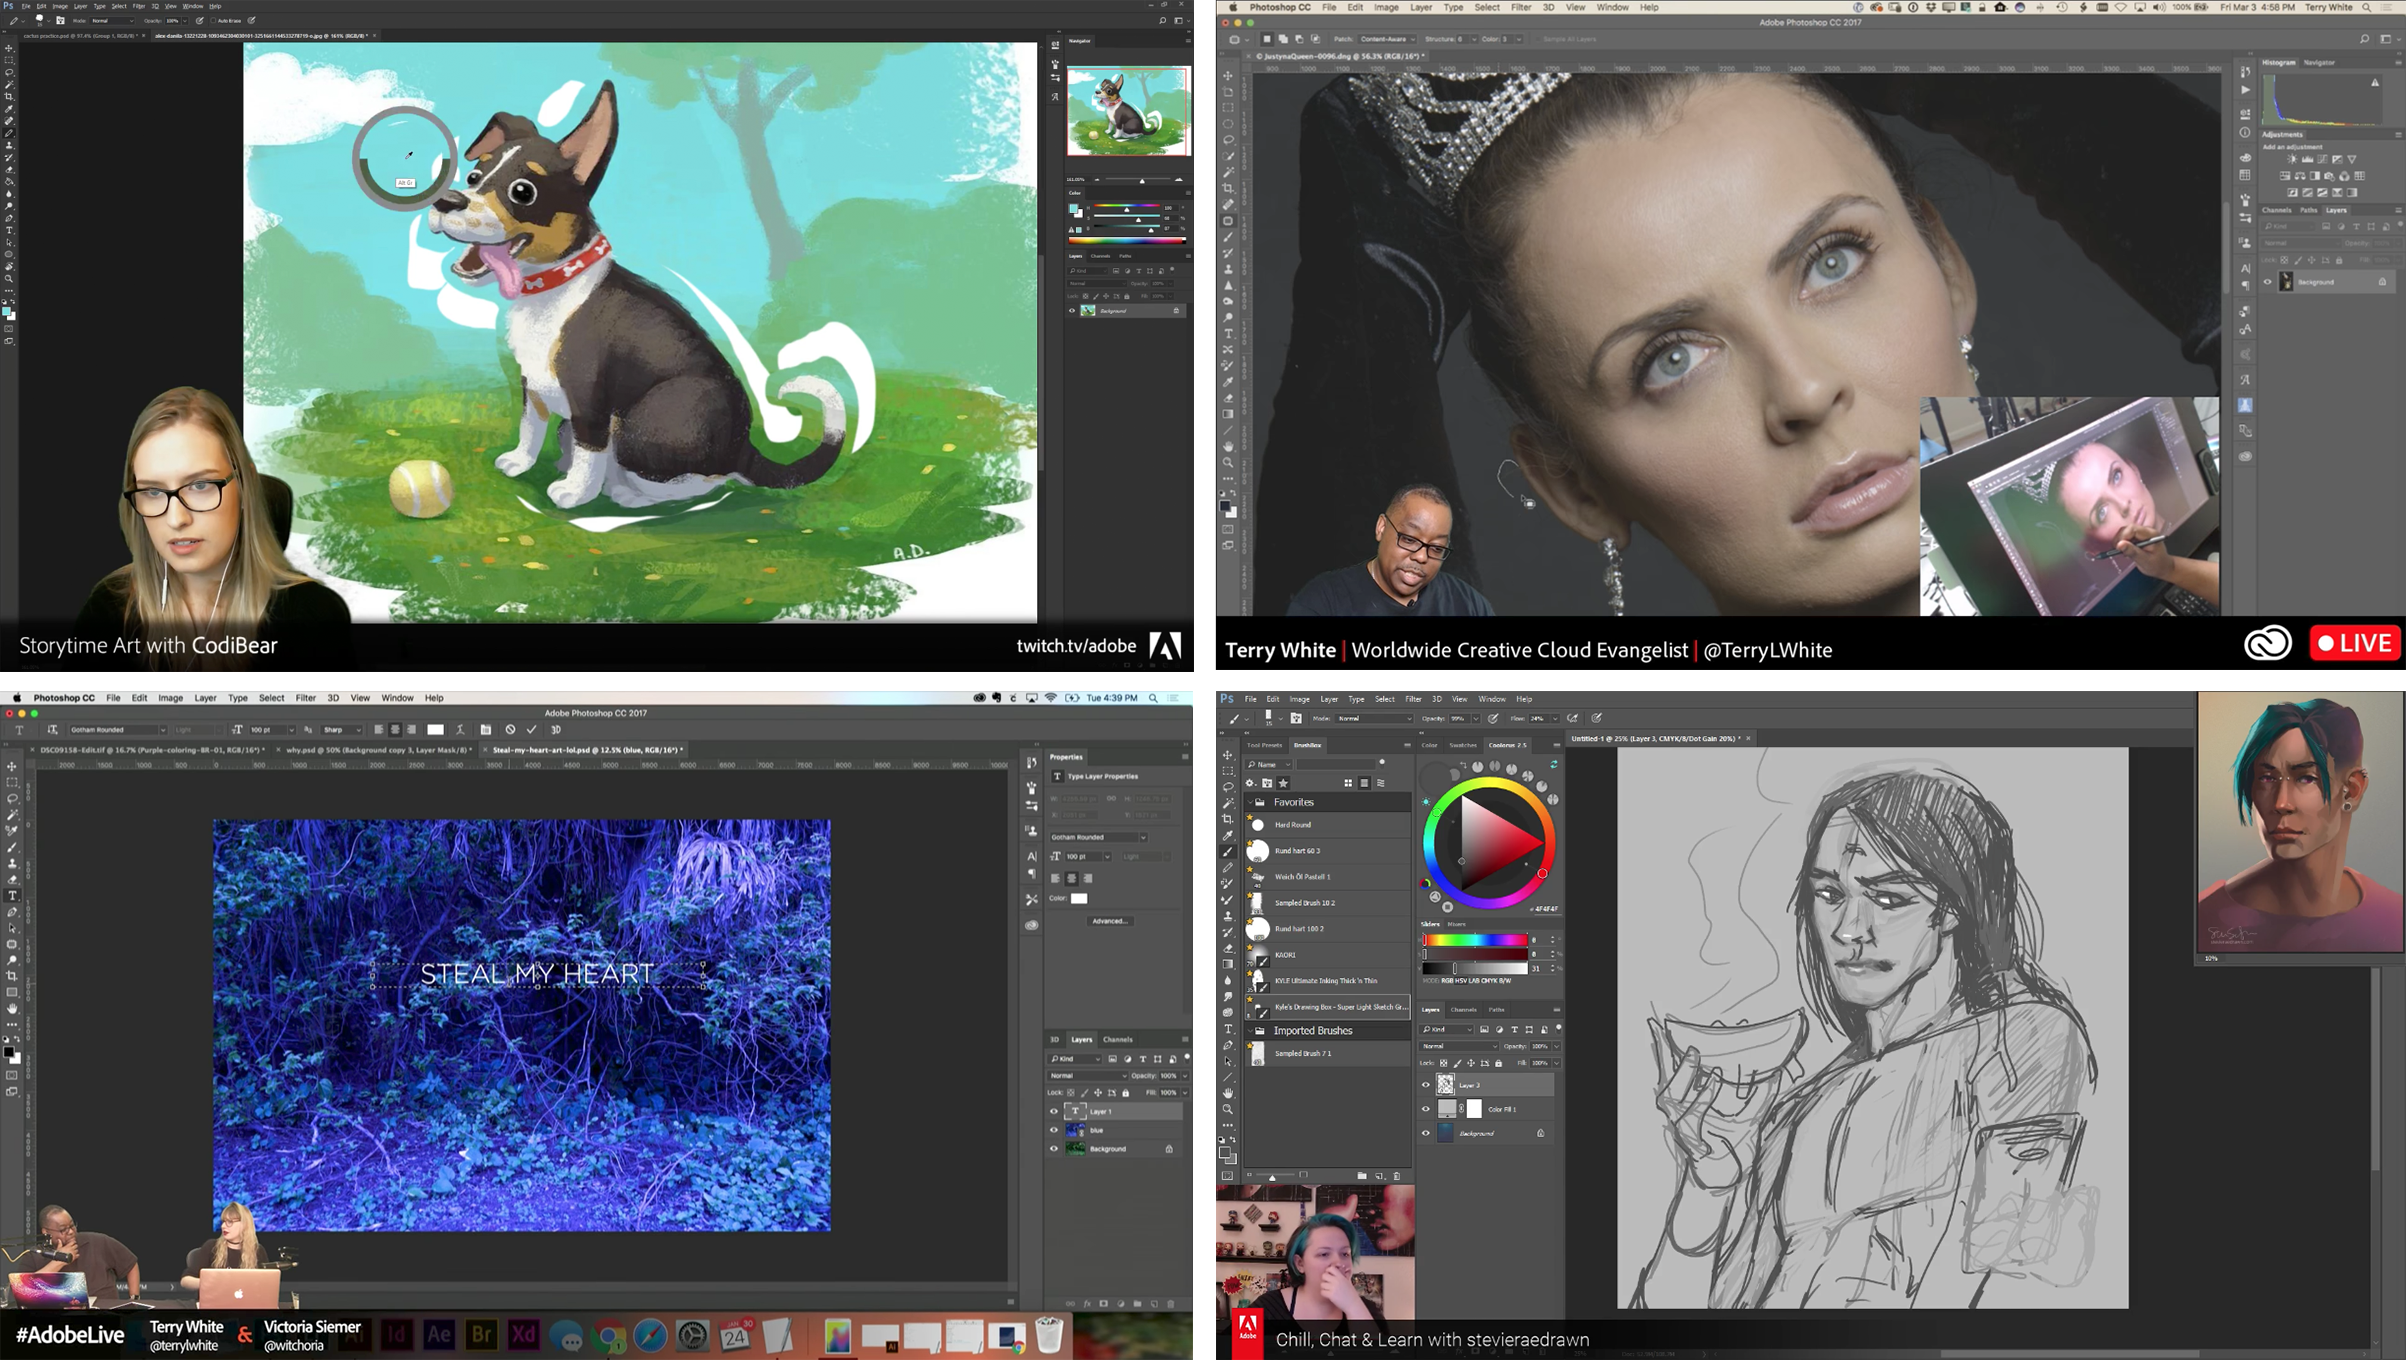
\includegraphics[width=\columnwidth]{liveclips/figures/streamers.png}
%   \caption{Examples of creative live streams on Twitch and YouTube. Artists stream videos of themselves working on creative projects such as graphic design, illustration, and photo editing. (Sources for video screenshots: top left\protect\footnotemark, top right\protect\footnotemark, bottom left\protect\footnotemark, bottom right\protect\footnotemark)}~\label{fig:liveclips_streamers}
% \end{figure}

\subsection{Segmenting Videos to Make Them More Browsable}
This work uses videos as the source for inspirational examples. Videos have the advantage over text and static images that they show the process of using a tool, rather than just the outcome, and they provide visual demonstrations that are directly relatable to the visual user interface \cite{Grossman2010a}.

Extensive prior work has explored automatically generating educational video clips from screencast videos of software use \cite{Pongnumkul2011, Chi2012, Banovic2012, Lafreniere2014, Nguyen2015}. Though some methods rely on matching telemetry data for these videos \cite{Grossman2010, Lafreniere2014, Chi2012}, others have shown that computer vision alone can be used to detect tool selection events when such data is not available \cite{Pongnumkul2011, Banovic2012}. In this work, we use telemetry data to segment live streamed videos into clips and rely on computer vision for the presentation and ranking of clips. 

Given a long video with associated tool data, prior work suggests techniques for extracting clips that demonstrate particular tools \cite{Pongnumkul2011, Chi2012, Lafreniere2014}, and guidelines for selecting clips with the best learning value \cite{Lafreniere2014}. Lafreniere \textit{et al.}'s recommended guidelines \cite{Lafreniere2014} include keeping clips short (15-25 seconds), using clips that show clear visual change to the document, and avoiding clips that show multiple unrelated actions. LiveClips builds on this approach to extract and rank clips from live streamed videos and explores how the characteristics of an inspiring clip might differ from that of an instructional one.
